%!TEX root = ../../14-icra-RealTimeNMPC.tex

\newcommand{\tetazero}{20.55}
\newcommand{\Fkxzero}{-20}
\newcommand{\Fkyzero}{20}

\newcommand{\tetaone}{-20}
\newcommand{\Fkxone}{5}
\newcommand{\Fkyone}{0}

\newcommand{\tetatwo}{20}
\newcommand{\Fkxtwo}{25}
\newcommand{\Fkytwo}{20}

%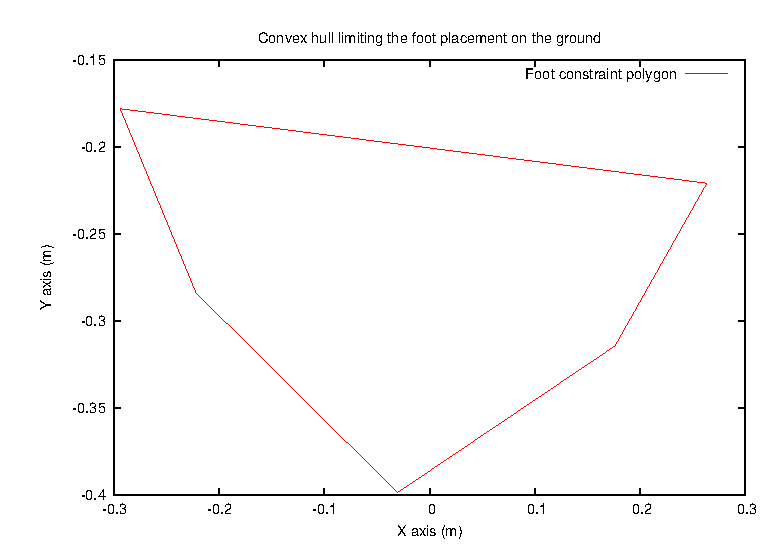
\includegraphics[width=15cm]{./figures/walking-without-thinking/ConvexHull}
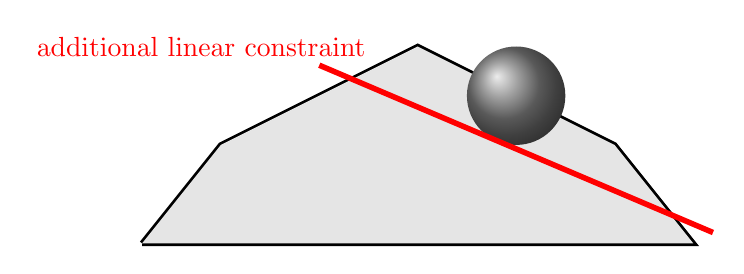
\begin{tikzpicture}[scale=0.125]
%\draw [dashed][->](-50,0) -- (50,0) node [below left, black]{$\overrightarrow{x}$}; %x-axis
%\draw [dashed][->](0,-50) -- (0,50) node [below left, black]{$\overrightarrow{y}$}; %y-axis
 %left support, right foot landing convexhull
\draw [line width=2pt](-28,20)--(-20,30)--(0,40)--(20,30)--(28,20)--(-28,20) node at (-10,30)[black]{} ;
\fill [color=gray!20,line width=2pt] (-28,20)--(-20,30)--(0,40)--(20,30)--(28,20)--(-28,20) ;
%pattern=north east lines
 %support foot
%\draw (-10,-5)--(10,-5)--(10,5)--(-10,5)--(-10,-5) node [below left, black]{Support Foot} ;

\shade[ball color=gray] (10,35) circle (5cm);

\draw [line width=2pt,red](-10,38.10)--(30,21.10) node at (-22,40)[red]{additional linear constraint} ;
\end{tikzpicture}

%
%\begin{tikzpicture}[x=0.7cm,y=0.7cm]
%\node (D) at (0,0) [coordinate] {} ;
%\node [below left] at (D) {D} ;
%\node (G) at (3,0) [coordinate] {} ;
%\node [below] at (G) {G} ;
%\node (C) at (5,0) [coordinate] {} ;
%\node [below right] at (C) {C} ;
%\node (F) at (5,3) [coordinate] {} ;
%\node [right] at (F) {F} ;
%\node (B) at (5,5) [coordinate] {} ;
%\node [above right] at (B) {B} ;
%\node (E) at (2,5) [coordinate] {} ;
%\node [above] at (E) {E} ;
%\node (A) at (0,5) [coordinate] {} ;
%\node [above left] at (A) {A} ;
%\node (H) at (0,2) [coordinate] {} ;
%\node [left] at (H) {H} ;
%\filldraw[color=lightgray] (D) -- (G) -- (H) ;
%\filldraw[color=lightgray] (G) -- (C) -- (F) ;
%\filldraw[color=lightgray] (F) -- (B) -- (E) ;
%\filldraw[color=lightgray] (E) -- (A) -- (H) ;
%\draw (D) -- node[below] {$b$} (G) -- node[below] {$a$} (C) ;
%\draw (C) -- node[right] {$b$} (F) -- node[right] {$a$} (B) ;
%\draw (B) -- node[above] {$b$} (E) -- node[above] {$a$} (A) ;
%\draw (A) -- node[left] {$b$} (H) -- node[left] {$a$} (D) ;
%\draw (G) -- (F) ;
%\draw (F) -- (E) ;
%\draw (E) -- (H) ;
%\draw (H) -- (G) ;
%\end{tikzpicture}
%
%
%
%
%\begin{tikzpicture}[x=0.7cm,y=0.7cm]
%\node (D) at (0,0) [coordinate] {} ;
%\node [below left] at (D) {D} ;
%\node (G) at (3,0) [coordinate] {} ;
%\node [below] at (G) {G} ;
%\node (C) at (5,0) [coordinate] {} ;
%\node [below right] at (C) {C} ;
%\node (F) at (5,3) [coordinate] {} ;
%\node [right] at (F) {F} ;
%\node (B) at (5,5) [coordinate] {} ;
%\node [above right] at (B) {B} ;
%\node (E) at (2,5) [coordinate] {} ;
%\node [above] at (E) {E} ;
%\node (A) at (0,5) [coordinate] {} ;
%\node [above left] at (A) {A} ;
%\node (H) at (0,2) [coordinate] {} ;
%\node [left] at (H) {H} ;
%
%\filldraw[color=lightgray,pattern=crosshatch] (G) -- (C) -- (F) ;
%\filldraw[color=lightgray,pattern=crosshatch] (F) -- (B) -- (E) ;
%\filldraw[color=lightgray,pattern=crosshatch] (E) -- (A) -- (H) ;
%\draw (D) -- node[below] {$b$} (G) -- node[below] {$a$} (C) ;
%\draw (C) -- node[right] {$b$} (F) -- node[right] {$a$} (B) ;
%\draw (B) -- node[above] {$b$} (E) -- node[above] {$a$} (A) ;
%\draw (A) -- node[left] {$b$} (H) -- node[left] {$a$} (D) ;
%\draw (G) -- (F) ;
%\draw (F) -- (E) ;
%\draw (E) -- (H) ;
%\draw (H) -- (G) ;
%\end{tikzpicture}
